\documentclass[a4paper, 12pt]{article}
\usepackage[utf8]{inputenc}
\usepackage[T1]{fontenc}
\usepackage{textcomp, color, amsmath, amssymb, tikz, subfig, float, mathrsfs}
\usepackage{xcolor}
\usepackage{amsfonts}
\usepackage{graphicx}
\usepackage{listings}
\usepackage{ragged2e}
\usepackage{amsmath}
\usepackage[export]{adjustbox}
\usepackage[]{esint}
\usepackage{hyperref}
\usepackage[skins,theorems]{tcolorbox}
\usepackage{cite}
\usepackage{algorithm}
\usepackage{algorithmicx}
\usepackage{algpseudocode}
\usepackage{subfig}% http://ctan.org/pkg/subfig
\usepackage{hyperref}
\usepackage{setspace}
\newsubfloat{figure}


%Tikzcommands
\usepackage{tikz}
\usetikzlibrary{shapes.geometric, arrows}
\tikzstyle{startstop} = [rectangle, rounded corners, minimum width=3cm, minimum height=1cm,text centered, draw=black, fill=red!30]
\tikzstyle{io} = [trapezium, trapezium left angle=70, trapezium right angle=110, minimum width=3cm, minimum height=1cm, text centered, draw=black, fill=blue!30]
\tikzstyle{process} = [rectangle, minimum width=3cm, minimum height=1cm, text centered, draw=black, fill=orange!30]
\tikzstyle{decision} = [diamond, minimum width=3cm, minimum height=1cm, text centered, draw=black, fill=green!30]
\tikzstyle{arrow} = [thick,->,>=stealth]



\tcbset{highlight math style={enhanced,
  colframe=red,colback=white,arc=10pt,boxrule=0.5pt, hbox}}

\definecolor{lightgray}{gray}{0.75}

\newcommand\greybox[1]{%
  \vskip\baselineskip%
  \par\noindent\colorbox{lightgray}{%
    \begin{minipage}{\textwidth}#1\end{minipage}%
  }%
  \vskip\baselineskip%
}
	
\newcommand{\vertfig}[2][]{%
  \begin{minipage}{.5\textwidth}
  \centering
  \subfloat[#1]{\includegraphics[width=\textwidth]{#2}}
  \end{minipage}}
  
\newcommand{\horizfig}[2][]{%
  \begin{minipage}{.5\textwidth}\subfloat[#1]{\includegraphics[width=.5\textwidth]{#2}}\end{minipage}}

\linespread{1.5}
\begin{document}



\author{Kristian Tuv}
\title{FYS3710  Cellelab}
\maketitle

\section{Innledning}
Vi har i dette eksperimentet brukt et flowcytometer til å måle DNA mengdene i celler som har blitt bestrålet med 1 Grey og 5 Grey, samt å måle DNA mengden i celler som ikke er bestrålt som kontroll.

\section{Teori}
Ved bestråling av celler av normale celler i kroppen, vil enten cellene forsøke å reparere seg selv eller begå selvmord ved apoptose, og dermed omdannes til mat for for nabocellene. Det kan ofte være bedre å la de skadede cellene gå inn i apoptose enn å reprarer skader, som kan føre til feil under reparasjonen og senere mutasjon og kreftutvikling.\\
For at cellen skal kunne gå inn i mitose og dele seg, er det flere checkpointer i celledelingssyklusen cellen må komme seg igjennom. Dette er for å sikre at celler med skader på DNA deler seg.\\
Vi kan dele cellesyklusen inn i 4 deler, se figur 1. Dersom cellen rekker frem til mitose før den dør vil dette kunne føre til nekrose, cellesprekking og toksisek produkter. \\

\begin{figure}[H]
\centering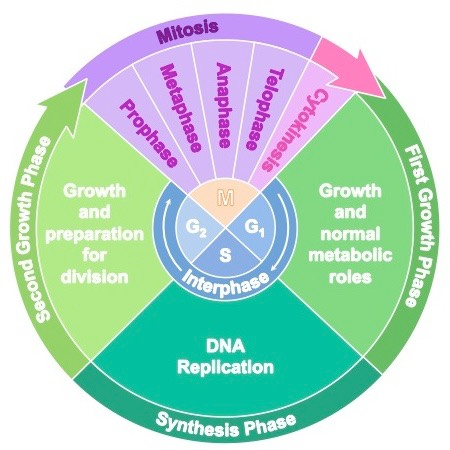
\includegraphics[scale=.8]{cellelab.jpg}
\caption{Illustrasjon av cellesyklusen delt inn i 4 faser.\\ G1: Vanlig vekst. \\S: DNAet dobles.\\ G2: Videre vekst of forberedelse til celledeling.\\ M: Cellen deles.\\
En cellesyklus tar ca 24 timer, der cellen befinner seg mesteparten av tiden i fase G1.\\
Kilde:\url{http://ib.bioninja.com.au/standard-level/topic-1-cell-biology/16-cell-division/cell-cycle.html}, 15.11.2017}
\end{figure}


\section{Flowcytometer}
I flowcytometeret sendes cellene ekeltvis forbi en lasterstråle som kan eksitere flourescerende stoffer. Cellen har på forhånd blitt merket med propidium iodid (PI), som er et flourescerende stoff som binder seg til DNA. PI eksiteres og sender ut lys når stoffet deeksiteres. Vi bruker metoden til å måle DNA mengden i en celle, og utifra hvor mye DNA det er vet vi også hvilken fase av cellesyklusen cellen er i.

\section{Gjennomføring}
6 flasker med mellom 0.5 og 1 million celler analyseres. 
\begin{itemize}
\item 2 flasker er kontrollflasker
\item 2 flasker bestråles med 1 Gy på 220 kV
\item 2 flasker bestråles med 5 Gy på 220 kV
\end{itemize} 
\textbf{Prosedyre}:\\
Dagen før:
\begin{itemize}
\item Cellene bestråles med 220 keV røntgen og inkuberes i 4 timer
\item Cellene trypsineres og sentrifugeres
\item Vaskes 2 ganger med 5 ml PBS og sentrifugeres
\item Pellet resuspenderes i 200 $\mu$l PBS, vortex. 5 ml fyserkald 70 \% ethanol tilsettes drålevis. 24-48 timer i kjøleskap.
\end{itemize}
På dagen:
\begin{itemize}
\item Alle prlver setrifugeres og vaskes 2 ganger i PBS
\item Sentrifugeres og resuspenderes i 500 $\mu$l PBS med 35 $\mu$g Pl + 100 $\mu$g/ml RNAse
\item Vente i 45 min med prøvene i mørkt rom
\item Prøvene filtreres og kjøres på flowcytometer
\end{itemize}
\section{Resultater}

\begin{figure}[H]
\vertfig[Kontroll 1]{/Users/Tuv/Documents/UiO/H17/FYS3710/Cellelab/Results/kontroll-1.png}
\vertfig[Kontroll 2]{/Users/Tuv/Documents/UiO/H17/FYS3710/Cellelab/Results/kontroll-2.png}
\caption{Kontrollprøver. Vi ser her at antall celler i G1 fase (første topp) er langt større en antall celler i G2 fase (andre topp)}
\end{figure}
\begin{figure}[H]
\vertfig[1Grey 1]{/Users/Tuv/Documents/UiO/H17/FYS3710/Cellelab/Results/1grey-1.png}
\vertfig[1Grey 2]{/Users/Tuv/Documents/UiO/H17/FYS3710/Cellelab/Results/1grey-2.png}
\caption{Prøver bestrålt med 1 Gy. Vi ser her at forholdet mellom antall celler i G1 fase og G2 fase har sunket sammenlignet med kontrollprøvene}
\end{figure}
\begin{figure}[H]
\vertfig[5 Grey 1]{/Users/Tuv/Documents/UiO/H17/FYS3710/Cellelab/Results/5grey-1.png}
\vertfig[5 Grey 2]{/Users/Tuv/Documents/UiO/H17/FYS3710/Cellelab/Results/5grey-2.png}
\caption{Prøver bestrålt med 5 Gy. Vi ser her at forholdet mellom antall celler i G1 fase og G2 fase har sunket sammenlignet med kontrollprøvene}
\end{figure}

\begin{figure}[H]
\begin{center}
\begin{tabular}{ |c|c|c|c| }
\hline
Prøve & \% G1 & \%  S &  \% G2\\
\hline
Kontroll 1 & 51.743 & 33.671 & 14.586\\ \hline
Kontroll 2 & 52.978 & 32.864 & 14.159\\\hline
1 Grey 1 & 40.548 & 35.539 & 23.913 \\\hline
1 Grey 2 & 44.261 & 40.660 & 15.079 \\\hline
5 Grey 1 & 37.268 & 45.466 & 17.266 \\\hline
5 Grey 2 & 43.638 & 35.772 & 20. 371 \\
\hline
\end{tabular}
\caption{Tabell over prøveresultater. Antall celler i hver fase er oppgitt i prosent}
\end{center}
\end{figure}
\section{Diskusjon og konklusjon}
Fra tabellen i Figur 5 ser vi at kontrollprøven har flest celler i G1 fase. Dette stemmer godt med hva vi bør forvente, siden kontrollprøvene ikke har blitt bestrålt, og de aller fleste cellene derfor bør gå igjennom cellesyklusen uten problemer og starte på en ny cellesyklus. Siden G1-fasen tar lengst tid, er det også å forvente at de fleste cellene befinner seg i denne fasen.\\
For prøvene som har blitt bestrålt ser vi at antall celler i G1 fase synker desto mere vi har bestrålt prøvene. For S fase og G2 fase ser vi at antallet celler stiger fordi de bestrålte cellene stanser sin cellesyklus for å enten kunne reparere cellen eller kunen gå inn i apoptose.

\end{document} 